\documentclass{article}

\usepackage{times}
\usepackage{graphicx}
\usepackage{subfigure}
\usepackage{natbib}
\usepackage{algorithm}
\usepackage{algorithmic}
\usepackage{lipsum}
\usepackage{todonotes}
\usepackage[accepted]{icml2017}
\icmltitlerunning{CS 281 Final Project Template}

\begin{document}

\twocolumn[
\icmltitle{Using Non-Task Data To Solve Cold Start Problems in Heterogeneous Peer Prediction}
\begin{icmlauthorlist}
\icmlauthor{Brian Hentschel}{}
  \icmlauthor{Anna S. Hilgard}{}
\icmlauthor{Casey Meehan}{}
\end{icmlauthorlist}

\vskip 0.3in
]

\begin{abstract}
  \begin{itemize}
  \item This document describes the expected style, structure, and rough proportions for your final project write-up.
  \item While you are free to break from this structure, consider it a strong prior for our expectations of the final report.
\item Length is a hard constraint. You are only allowed max \textbf{8 pages} in this format. While you can include supplementary material, it will not be factored into the grading process. It is your responsibility to convey the main contributions of the work in the length given.
  \end{itemize}


\lipsum[1]
\end{abstract}

\section{Introduction}
\label{sec:introduction}

%Example Structure:
%\begin{itemize}
%\item What is the problem of interest and what (high-level) are the current best methods for solving it?
%\item How do you plan to improve/understand/modify this or related methods?
%\item Preview your research process, list the contributions you made, and summarize your experimental findings.
%\end{itemize}

In peer prediction settings with heterogeneous users, the goal is to make truthful reporting a low-regret strategy for any agent. To fully minimize expected regret while allowing for heterogeneity, this would require the computation and use of individualized user-user signal correlations for every pair of users. This is in general computationally infeasible, so methodologies typically focus instead on clustering similar users while trying to minimally distort their individual signal distributions. 

Additionally, because this method explicitly requires an existing signal distribution, there is a cold start problem: if we do not already have a significant amount of task data for a new user, we cannot know how properly to reward them in comparison to their peers. In our project, we focus on two specific goals:
\begin{enumerate}
\item Clustering is usually done by comparing each user`s reports with other users. We aim to speed up this clustering by using latent variable matrix factorization and then clustering on much smaller latent variables.
\item Bootstrapping the clustering process by using non-task data to form an initial clustering before agent reporting begins.
\end{enumerate}

\section{Background}
%Example Structure:
%\begin{itemize}
%\item What information does a non-expert need to know about the problem domain?
%\item What data exists for this problem?
%\item What are the challenges/opportunities inherent to the data? (High dimensional, sparse, missing data, noise, structure, discrete/continuous, etc?)
%\end{itemize}

In \citet{shnayder2016informed}, Shnayder et al. prove that the Correlated Agreement multi-task peer prediction mechanism maximally incentivizes truthful reporting without a ground truth for homogeneous users. The CA mechanism can be generalized to non-homogeneous users but requires a prohibitive number of user reports; thus, \citet{agarwal2017} bounds expected regret by clustering users with similar signal-report distributions.  This regret bound is proportional to the L1 difference between user-user '$\Delta$ Matrices' and those of their respective clusters, where a $\Delta$ Matrix of users $q,r$ is defined as: $$D_{q,r}(i,j) = p(\textrm{q reports i, r reports j}) - p(\textrm{q reports i})p(\textrm{r reports j})$$
The primary dataset we use is that of the Good Judgment Global Forecasting Competition, available at \texttt{https://dataverse.harvard.edu/dataverse.}
\texttt{xhtml?alias=gjp}. There are many challenges inherent to this dataset. First, the idea of a task is not well-defined. Users enter predictions in continuous time, and the true probability of an event will change over time, such that each minute could be considered a different task (Note that if we expect users only update their predictions in response to new information, these time-question tasks will be independent conditional on the signal). We choose to bucket these responses by week to mediate between the desire to allow for variation in true probability over time while maintaining sufficient task response density. This results in 1,499,294 predictions by 2,052 users on 1,548 tasks. Secondly, the signal itself can be expected to have a high degree of noise, as the probability of any of these global events is not well-defined even in the absence of individual interpretation effects. 

To study the effects of the clustering methodologies in a slightly less noisy realm, we additionally use a second dataset of user judgments on whether or not websites contained adult content. This dataset, termed \emph{Adult}, was pulled from the Square Project at the University of Texas. The data is available at \texttt{https://github.com/ipeirotis/}
\texttt{Get-Another-Label/tree/master/data}. We limit the dataset to users who gave at least one report of each signal, resulting in 65,144 reports by 389 users on 10,381 tasks.

Both datasets required significant preprocessing to account for sparsity of signal distributions and to compute the $\Delta$ matrices. Additionally, because Good Judgment reports were continuous rather than discrete, we bucketed the responses into five uniform bins, which we use to compute the matrices.

\section{Related Work}

%Example Structure:
%\begin{itemize}
%\item What 3-5 papers have been published in this space?
%\item How do these  differ from your approach?
%\item What data or methodologies do each of these works use?
%\item How do you plan to compare to these methods?
%\end{itemize}

\citep{agarwal2017} is the only paper we know of specifically considering clustering methods for heterogeneous peer prediction. The paper differs from our work in that it assumes all of the relevant data exists and seeks to prove a theoretical upper bound on regret rather than to study empirical average regret in settings with sparse data. While the authors also use the \emph{Adult} dataset among others, they restrict it to a small subset of only those users for whom there is a full joint distribution between any two users, resulting in only 269 users. 

Further, while the authors prove a theoretical bound in the case of empirically estimated ground truth, the tests they run on real data rely on the existence of a known ground truth label. This allows them to calculate individual signal confusion matrices using methods developed in \citet{dawid1979maximum} and leverage tensor decomposition techniques from \citet{anandkumar2014tensor} and \citet{zhang2016spectral} to compute average clusters directly. We seek to show that in the more general case of incomplete data with no ground truth labels, clustering instead on user-specific latent variables learned through matrix factorization can lead to similar computational savings as tensor decomposition while eliminating the need for labels.  Further, we show that these computationally efficient clusterings are similarly effective with respect to incentivizing truthfulness as clustering on $\Delta$ matrices directly.

The use of the Correlated Agreement mechanism \citep{shnayder2016informed} requires that the $\Delta$ matrices are already known or can be empirically estimated from observed data. Nothing in the peer prediction literature addresses this cold start problem yet. However, it is well studied in the field of matrix factorization. The most similar method to ours, in that it incorporates non-task data, is \citep{kula2015metadata}.


\section{Model}

%Example Structure:

%\begin{itemize}
%\item What is the formal definition of your problem?
%\item What is the precise mathematical model you are using to represent it? In almost all cases this will use the probabilistic language from class, e.g.
%  \begin{equation}
 % z \sim {\cal N}(0, \sigma^2)\label{eq:1}
%\end{equation}
%But it may also be a neural network, or a non-probabilistic loss,
%\[ h_t \gets \mathrm{RNN}(x_{t}, h_{t-1} )\]

%This is also a good place to reference a diagram such as Figure~\ref{fig:diagram}.

%\item What are the parameters or latent variables of this model that you plan on estimating or inferring? Be explicit. How many are there? Which are you assuming are given? How do these relate to the original problem description?
%\end{itemize}

Given a sparse matrix containing tasks, users, and users` reports on each task, the goal is to produce clusters which accurately describe users` reporting behavior. Because of the sparse matrix data, we focus on matrix factorization models to generate latent factor representations of users. That is, we assume that there is some latent variable representation of a user`s forecasting behavior, $u_i$ that interacts with related task-specific factors, $t_j$. These could be thought of, for example as the task`s topic areas and the user`s expertise in those specific topic areas. After transforming the predictions to range from -1 to 1 instead of 0 to 1, we use the following model, shown in Figure~\ref{fig:diagram}:  
  $$
  p_{i,j} \sim \mathcal{N}(\textrm{tanh}\left( \mu_{i_M}\left[u_i^{T}t_j + g + \mu_j\right] + \mu_{i_A}\right), \sigma^2)
 $$
 
 Users tend to exhibit two forms of individualized biases in this space. The multiplicative bias, $\mu_{i_A}$ captures either risk aversion or overconfidence, such that they tend to predict values either closer to or farther from 0 (.5) than are warranted by their knowledge. The additive bias, $ \mu_{i_M}$ captures both availability bias or normalcy bias which would result in user having a tendency to predict a specific level. The task bias $\mu_j$ captures the general prediction likelihood of the task absent user-specific factors, and the global bias $g$ captures the overall mean of the user-task predictions.
  The tanh restricts the space of the predicted mean to the domain of the target value.
  
  Then, we must infer $k+2$ parameters for each user, $k+1$ parameters for each task, and one global bias, where $k$ is the length of the latent vector representation we choose for users and tasks. Only the predictions $p_{i,j}$ are known in this model.
  
      For \emph{Adult}, which does not have this probablistic representation and has reports ranging from 1 to 4, we use only additive biases and remove the tanh.
      
  XX TODO PREDICTING LATENT USER VECTORS FROM PSYCH DATA XX

\begin{figure}
  \centering
  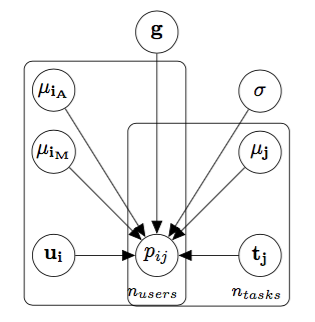
\includegraphics[height=8cm]{dgmaccurate.png}
  \caption{\label{fig:diagram} Model of prediction generation.}
\end{figure}


\section{Inference (or Training)}

%\begin{itemize}
%\item How do you plan on training your parameters / inferring the
%  states of your latent variables (MLE / MAP / Backprop / VI / EM / BP / ...)
%
%\item What are the assumptions implicit in this technique? Is it an approximation or exact? If it is an approximation what bound does it optimize?
%
%\item What is the explicit method / algorithm that you derive for learning these parameters?
%\end{itemize}

For learning the latent user parameters, we use mini-batch stochastic gradient descent to find the maximum likelihood estimate. We choose not to use a prior for regularization as we find that the training and validation performance do not generally diverge. This is likely because there is already enough noise in the training data for each parameter that it is difficult to overfit the model. We do not explicitly code the initialization of the model, so of course it is possible it finds a local rather than global minimum. However, the performance of the model is consistent across random starts.

\begin{algorithm}
  \begin{algorithmic}
  \STATE {learning rate = $\alpha$}
  \FOR{\textrm{epoch in epochs} }
  \FOR{\textrm{batch in batches} }
    \STATE{Calculate the gradient of the MSE Loss for each parameter for all users and tasks in the batch}
    \STATE{Update the parameters: param $\gets$ param - $\alpha$ * $\frac{d}{dparam}$(MSE Loss) }    
    \ENDFOR
    \ENDFOR
  \end{algorithmic}
  \caption{Mini-Batch SGD Parameter Fitting}
\end{algorithm}

TODO COLD START MODEL


\section{Methods}

\begin{itemize}
\item What are the exact details of the dataset that you used? (Number of data points / standard or non-standard / synthetic or real / exact form of the data)

\item What are the exact details of the features you computed?

\item How did you train or run inference? (Optimization method / hyperparameter settings / amount of time ran / what did you implement versus borrow / how were baselines computed).

\item What are the exact details of the metric used?
\end{itemize}

For the Good Judgment Dataset, we use the file \texttt{survey_fcasts.yr4.tab}, consisting of all user forecasts for the fourth year of the tournament. The file has 1,685,784 lines, each consisting of details about a specific user id and forecast. We restrict to only binary valued questions, for which a single probability of `yes' is given as the answer (as opposed to, for example, ``Who will be inaugurated as President of Russia in 2012?", which had 3 possible answers). We restrict to only users who responded to at least 30 Individual Forecasting Problems (IFPs) over the course of the year. Given that users can (and ideally do) update their predictions for IFPs over time, any given time period could be thought of as a new IFP. Following the scoring procedure of the Good Judgment, we assume that if a user enters a prediction and then does not update it, this implies that they would like their existing prediction to be carried forward.

\section{Results}

\begin{itemize}
\item What were the results comparing previous work / baseline systems / your systems on the main task?
\item What were the secondary results comparing the variants of your system?
\item This section should be fact based and relatively dry. What happened, what was significant?
\end{itemize}

\begin{table*}
  \centering
  \missingfigure{}
  \caption{This is usually a table. Tables with numbers are generally easier to read than graphs, so prefer when possible.}
  \label{fig:mainres}
\end{table*}


\begin{table}
  \centering
  \missingfigure[figheight=5cm]{}
  \caption{Secondary table or figure in results section.}
  \label{fig:mainres}
\end{table}

\lipsum[7-11]

\section{Discussion}



\begin{itemize}
\item What conclusions can you draw from the results section?
\item Is there further analysis you can do into the results of the system? Here is a good place to include visualizations, graphs, qualitative analysis of your results.

\item  What questions remain open? What did you think might work, but did not?
\end{itemize}

\lipsum[4-8]

\begin{figure}
  \centering
  \missingfigure{}
  \missingfigure{}
  \missingfigure{}
  \caption{Visualizations of the internals of the system.}
\end{figure}

\section{Conclusion}

\begin{itemize}
\item What happened?
\item What next?
\end{itemize}

\lipsum[4-6]

% \section*{Acknowledgements}

% \textbf{Do not} include acknowledgements in the initial version of
% the paper submitted for blind review.

% If a paper is accepted, the final camera-ready version can (and
% probably should) include acknowledgements. In this case, please
% place such acknowledgements in an unnumbered section at the
% end of the paper. Typically, this will include thanks to reviewers
% who gave useful comments, to colleagues who contributed to the ideas,
% and to funding agencies and corporate sponsors that provided financial
% support.


\bibliography{example}
\bibliographystyle{icml2017}

\end{document}
